\textbf{Autopilot and ground station}

\subsection{Overview}

In order for the multirotor to be controllable by a human being with minimal training, much of the flight systems need to be automated. We have decided for our project to use an open source autopilot called ‘Ardupilot’. The autopilot system consists of several hardware components and 2 software components which are split between the multirotor and the ground station.

\underline{Multirotor hardware}\

\begin{enumerate}

    \item Autopilot flight computer: The autopilot flight computer is the primary hardware component of the autopilot system on the multirotor. In the Ardupilot literature this device is referred to only as the ‘Autopilot’ but to avoid confusion with the broader autopilot system we will be referring to it as the ‘Autopilot flight computer’. The specific board that we are using is the APM 2.6. This board an older model and will thus be using legacy code but will have all of the required functionality.
  
  \item GPS and Compass: The GPS and compass will allow the ground station to track the multirotor while it’s flying. Also enables the use of the automatic flight modes.
 
 \item Telemetry module: Radio transceiver that allows for communication with the ground.
 
\end{enumerate}

\underline{Multirotor Software}

The autopilot flight computer uses open source software that the arudpilot website refers to as ‘firmware’. Because the board is an older version it actually does not have enough physical memory to fit the latest iterations of the firmware. As such we are using a legacy version of the firmware on our autopilot flight computer.

\underline{Ground station hardware}

The hardware for the ground station that is relevant to the autopilot is simply a computer and a telemetry system that will allow communication between the ground station and the multirotor.

\underline{Ground station software}

The ground station uses open source software called APM planner 2.0. The software is downloaded onto a laptop and provides the display, means of controller, and means of interfacing with the autopilot, including uploading the firmware.

\subsection{Features list}

\begin{enumerate}

    \item Real time monitoring of telemetry information: Data includes the altitude, position and orientation of the multirotor as well as real-time battery monitoring
    
    \item Real-time control of the Multirotor: Multirotor can be controlled either manually or by setting waypoints for it to follow or sending simple commands
    
    \item Primary Flight Display (HUD): Flight display is as appears below
    
\begin{figure}[H]
	\centering
	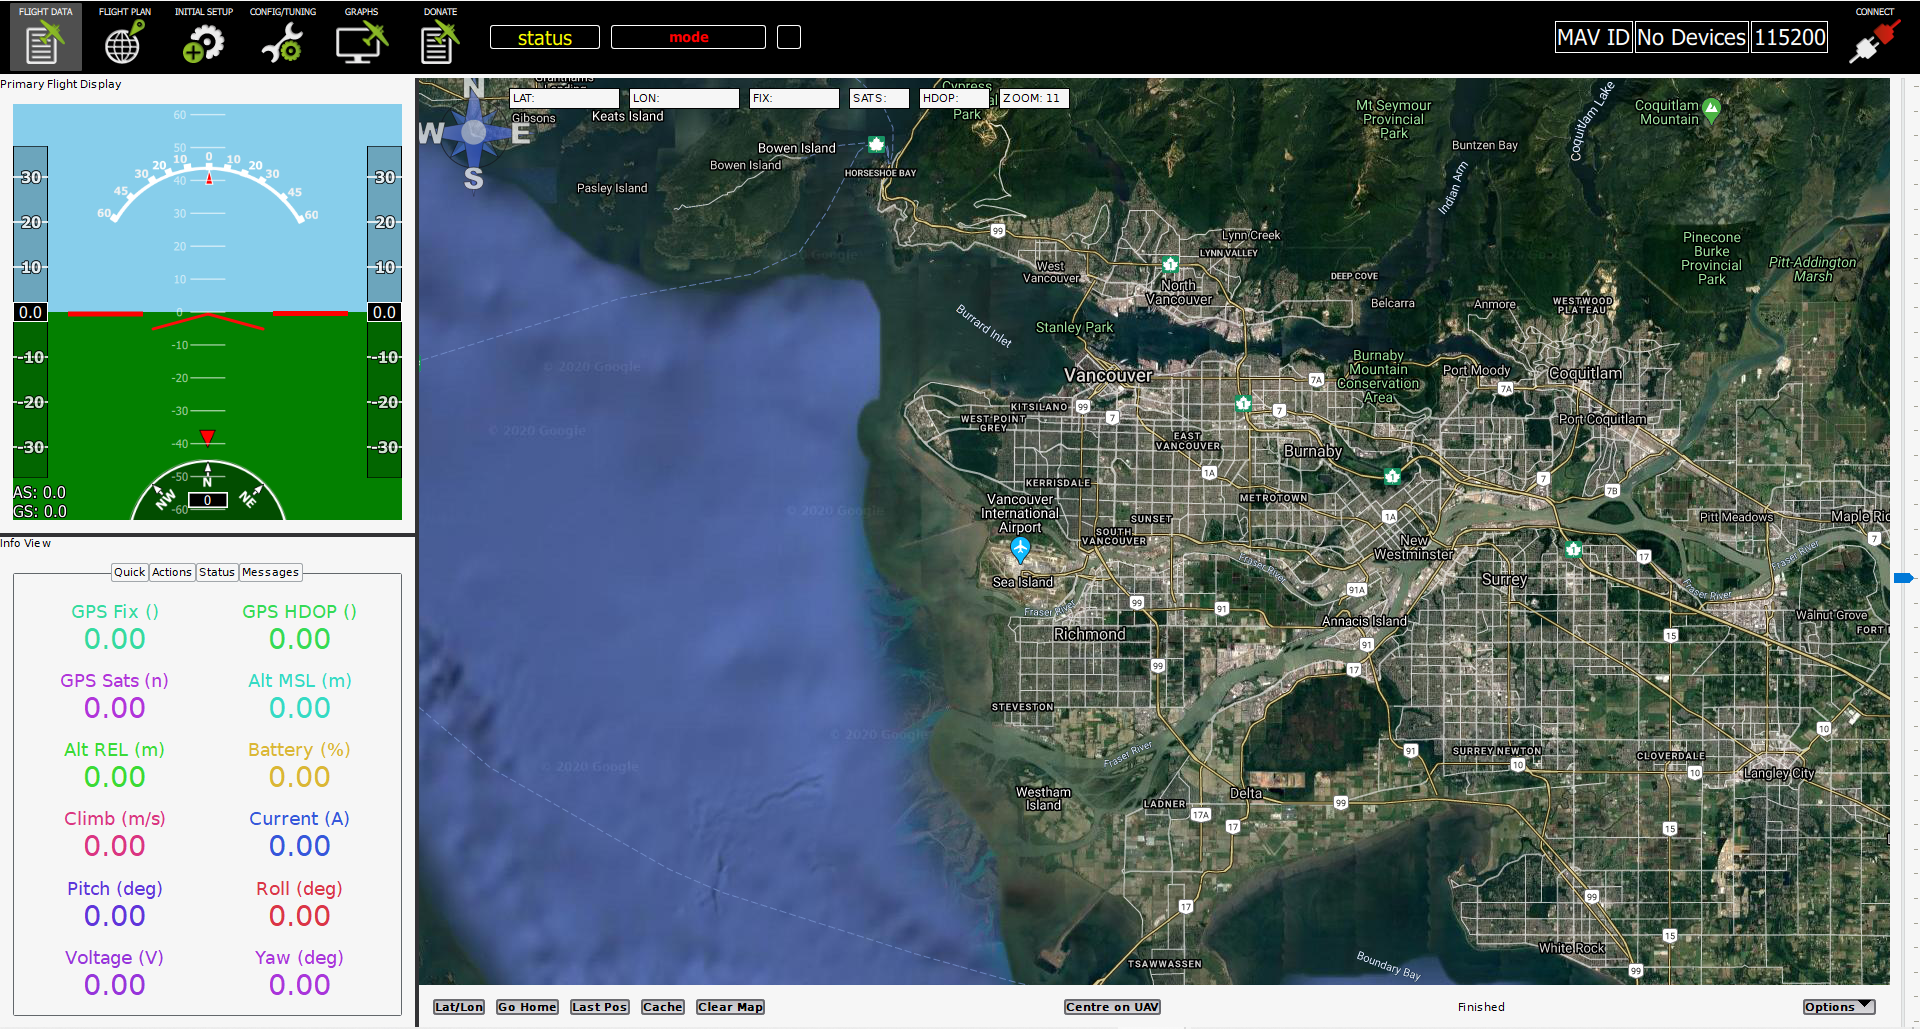
\includegraphics[width=15cm]{img/HUD.png}
	\caption{Flight display}
	\label{flight display}
	\end{figure}

    \item Simple commands to the Multirotor such as hover: These commands can be used in place of real-time control
    
    \item Waypoints that can be used to set a path for the multirotor to fly: Multirotor can fly a pre-programmed path by setting waypoints.
    
\end{enumerate}

\underline{Non-exhaustive list of Flight modes}

\begin{enumerate}

    \item Stabilize: Self-levels the roll and pitch axis
    
    \item Alt hold: Holds altitude and self-levels the roll and pitch axis
    
    \item Loiter: Holds altitude and position using GPS
    
    \item RTL: Returns to the takeoff position
    
    \item Stabilize: Self-levels the roll and pitch axis
    
    \item Auto: Executes pre-defined mission using waypoints
    
\end{enumerate}


